\section{Desenvolvimento do \textit{Software}}

A metodologia adotada combina fundamentos da engenharia química com técnicas modernas de desenvolvimento de \textit{software}, visando garantir precisão nos cálculos e acessibilidade por meio de uma interface \textit{web} intuitiva. O projeto foi estruturado em etapas que abrangem desde o levantamento bibliográfico das equações de dimensionamento até a implementação e validação do sistema completo. Para fins de organização, o desenvolvimento é descrito a seguir em seus principais eixos técnicos: \textit{backend}, \textit{frontend}, \textit{deploy}, automação de integração e entrega, distribuição \textit{desktop} e versionamento.

\subsection{\textit{Backend}}

O \textit{backend} foi desenvolvido em \textit{Python}, utilizando o \textit{framework} \textit{FastAPI}, escolhido por sua alta \textit{performance}, suporte a tipagem forte e facilidade na criação de \textit{APIs RESTful}. Essa camada é responsável por processar os cálculos, gerenciar as rotas de comunicação (\textit{endpoints}) e servir os resultados ao \textit{frontend}. Além disso, por se tratar de uma linguagem de alto nível, sua sintaxe é simples e intuitiva para iniciantes.

A Tabela \ref{tab:backend_libs} resume as principais bibliotecas e \textit{frameworks} utilizados, sua funcionalidade e a correspondência com aplicações típicas da engenharia química.

\begin{longtable}{|>{\raggedright\arraybackslash}p{0.2\textwidth}|>{\raggedright\arraybackslash}p{0.35\textwidth}|>{\raggedright\arraybackslash}p{0.35\textwidth}|}
\caption{Bibliotecas e \textit{frameworks} utilizados no \textit{backend}}
\label{tab:backend_libs} \\
\hline
\textbf{Nome} & \textbf{Funcionalidade} & \textbf{Como se enquadra no uso da Engenharia Química} \\ \hline
\endfirsthead
\caption[]{Bibliotecas e \textit{frameworks} utilizados no \textit{backend} (continuação)} \\
\hline
\textbf{Nome} & \textbf{Funcionalidade} & \textbf{Como se enquadra no uso da Engenharia Química} \\ \hline
\endhead
\hline
\multicolumn{3}{r}{\footnotesize{(Continua na próxima página)}} \\
\endfoot
\hline
\multicolumn{3}{c}{\footnotesize Fonte: Elaboração própria (2026).}
\endlastfoot
\textit{FastAPI} & \textit{Framework} \textit{web} moderno para criação de \textit{APIs RESTful} em \textit{Python}, com validação automática de dados e documentação interativa. & \textit{Backend} para expor os cálculos de engenharia química através de \textit{endpoints} HTTP, permitindo que a interface \textit{web} ou outros sistemas acessem as funções de dimensionamento, balanço de massa, cálculos de reatores etc. \\ \hline
\textit{Uvicorn} & Servidor \textit{ASGI} para executar aplicações \textit{web} assíncronas em \textit{Python}. & Executa o servidor da \textit{API} \textit{FastAPI}, processando as requisições dos cálculos. \\ \hline
\textit{Pydantic} & Biblioteca para validação de dados e gerenciamento de configurações usando \textit{Python} \textit{type hints}. & Valida os dados de entrada dos cálculos (vazões, temperaturas, pressões, propriedades físicas etc.), garantindo que os parâmetros fornecidos estejam no formato e tipo corretos antes de executar os cálculos. \\ \hline
\textit{CoolProp} & Biblioteca especializada em propriedades termodinâmicas de fluidos, com banco de dados extenso de substâncias. & Cálculo de propriedades termodinâmicas (densidade, viscosidade, entalpia, entropia, calor específico etc.) de compostos e misturas. \\ \hline
\textit{Pint} & Gerenciamento de unidades físicas, conversões e cálculos dimensionais & Permite trabalhar com diferentes sistemas de unidades, garantindo consistência dimensional nos cálculos. \\ \hline
\textit{Matplotlib} & Biblioteca de visualização de dados e criação de gráficos 2D/3D. & Gera gráficos de processos químicos como curvas de reação, perfis de temperatura, diagramas de fases, curvas de bomba, e visualizações de resultados de simulações. \\ \hline
\textit{NumPy} & Biblioteca fundamental para computação científica com \textit{arrays} multidimensionais e operações matemáticas vetorizadas & Realiza cálculos matriciais, interpolações, operações vetoriais para balanços de massa e energia, resoluções de sistemas de equações lineares em processos químicos \\ \hline
\textit{SciPy} & Conjunto de algoritmos científicos para otimização, integração numérica, álgebra linear, estatística & Resolução de EDOs, otimiza processos químicos, realiza integrações numéricas para cálculos de conversão, ajuste de curvas experimentais \\ \hline
\textit{Pytest} & \textit{Framework} de testes, com suporte a testes unitários, testes de integração, \textit{fixtures}, parametrização e relatórios detalhados. & Permite validar automaticamente a confiabilidade dos cálculos de engenharia química, garantindo que equações, modelos matemáticos e rotinas numéricas estejam corretos e continuem funcionando após alterações no código. \\ \hline
\end{longtable}

\subsection{\textit{Frontend}}

O \textit{frontend} corresponde à interface gráfica do usuário, sendo a parte visual e interativa do sistema, acessada diretamente pelo navegador. Ele é responsável por exibir os resultados dos cálculos, receber dados de entrada e enviar as informações ao servidor (\textit{backend}).

O \textit{frontend} foi desenvolvido com \textit{React}, \textit{TypeScript} e \textit{Vite}, combinação que favorece a composição da interface em componentes reutilizáveis, a tipagem dos contratos entre formulários e serviços e um ciclo de desenvolvimento ágil para compilação e distribuição da aplicação. A camada de navegação é estruturada com \textit{React Router}, o que permite organizar os módulos de tubulações, escoamento, bombas, componentes, reatores, balanço de massa e glossário em rotas aninhadas e previsíveis, sob um mesmo \textit{shell} de aplicação.

Na camada visual, a aplicação utiliza \textit{Tailwind CSS} para estilização utilitária, em conjunto com primitivas acessíveis de \textit{@base-ui/react} e componentes compostos no padrão da biblioteca \textit{shadcn}. Os ícones são fornecidos por \textit{Lucide React}, as notificações rápidas utilizam \textit{Sonner} e a renderização matemática é realizada com \textit{KaTeX}, o que permite exibir expressões em \LaTeX{} diretamente no navegador. Para as visualizações, a interface adota predominantemente componentes vetoriais em \textit{SVG} especializados para o contexto de engenharia química, apoiados por uma camada compartilhada de grades, eixos, marcadores, rótulos numéricos e legendas coloridas. Com isso, diagramas como \textit{Moody}, \textit{Levenspiel}, \textit{McCabe-Thiele}, envelope de fase, curva de pressão de vapor e mapas de processo podem compartilhar contratos de dados e convenções visuais sem replicar a lógica de apresentação em cada página.

Na organização da experiência, a interface foi concebida como um painel educacional único, com navegação lateral persistente, página inicial orientada por trilhas de aprendizagem e áreas de acesso rápido aos principais módulos. A disposição dos elementos busca explicitar o propósito pedagógico de cada seção, reduzindo a fricção de uso e favorecendo a leitura imediata dos resultados, dos gráficos e dos indicadores de processo. A Figura \ref{fig:piping_interface} ilustra a interface de usuário desenvolvida para o módulo de \textit{Piping}, evidenciando as escolhas de \textit{design} descritas.

\begin{figure}[H]
    \centering
    \caption{Interface gráfica do módulo de cálculos de tubulação (\textit{Piping})}
    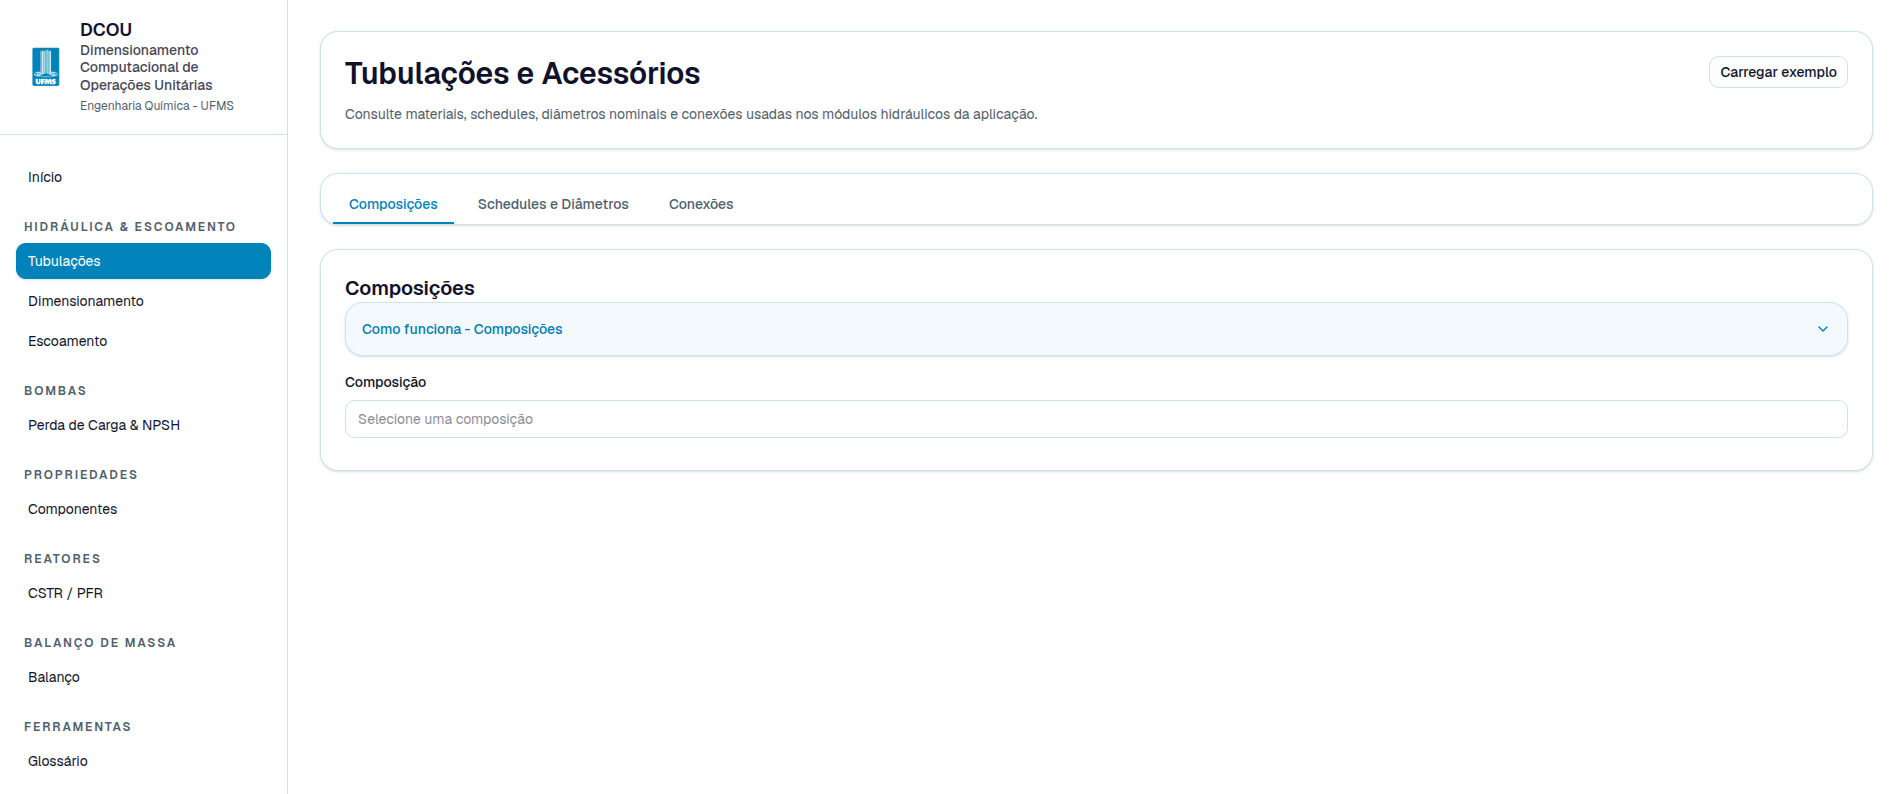
\includegraphics[width=\linewidth]{media/cap4_piping_interface.png}
    \fonte{Elaboração própria (2026).}
    \label{fig:piping_interface}
\end{figure}

\begin{table}[H]
\centering
\caption{Bibliotecas e \textit{frameworks} utilizados no \textit{frontend}}
\label{tab:frontend_libs}
\begin{tabular}{|>{\raggedright\arraybackslash}p{0.2\textwidth}|>{\raggedright\arraybackslash}p{0.7\textwidth}|}
\hline
\textbf{Nome} & \textbf{Funcionalidade} \\ \hline
\textit{Vite} & Ferramenta de \textit{build} e ambiente de desenvolvimento utilizada para empacotar a aplicação \textit{React}, com inicialização rápida e geração otimizada dos arquivos estáticos. \\ \hline
\textit{React} & Biblioteca declarativa para composição de interfaces em componentes reutilizáveis e encapsulados. \\ \hline
\textit{TypeScript} & Superset tipado de \textit{JavaScript} utilizado para formalizar contratos de dados, reduzir erros de integração e melhorar a manutenção. \\ \hline
\textit{React Router} & Biblioteca de roteamento usada para organizar os módulos do sistema em rotas navegáveis dentro da aplicação \textit{web}. \\ \hline
\textit{Tailwind CSS} & \textit{Framework} utilitário que facilita a criação de interfaces responsivas e personalizadas por meio de classes pré-definidas de estilo. \\ \hline
\textit{@base-ui/react} & Conjunto de primitivas acessíveis para construção de botões, diálogos, menus e outros controles de interface, sobre as quais são compostos os componentes visuais do sistema. \\ \hline
\textit{shadcn} & Camada de componentes reaproveitáveis, estilizados com utilitários e composta sobre primitivas acessíveis, empregada para estruturar cartões, botões, painéis e áreas de navegação. \\ \hline
\textit{Lucide React} & Biblioteca de ícones vetoriais modulares para navegação, estados visuais e ações contextuais na interface. \\ \hline
\textit{Sonner} & Biblioteca para notificações breves e não bloqueantes associadas às ações do usuário na interface. \\ \hline
\textit{KaTeX} & Biblioteca \textit{JavaScript} para renderização rápida de equações em \LaTeX{} diretamente no navegador. \\ \hline
\textit{Geist Variable} & Família tipográfica variável utilizada para padronizar a leitura visual e reforçar a identidade da interface. \\ \hline
\end{tabular}
\fonte{Elaboração própria (2026).}
\end{table}

Além da pilha principal, a interface utiliza uma camada de componentes visuais próprios para o contexto da Engenharia Química, incluindo cartões de módulo, painéis didáticos, blocos de métricas, indicadores de contexto e visualizações auxiliares para apoiar a interpretação dos fenômenos representados. Essa camada complementa a comunicação com a \textit{API} sem modificar os contratos de dados, ao mesmo tempo em que preserva a consistência visual e a legibilidade dos módulos. O mesmo \textit{frontend} também consome \textit{endpoints} de exemplo, o que permite pré-preencher entradas realistas para módulos como escoamento, dimensionamento, bombas e componentes antes da execução normal dos cálculos no \textit{backend}.

\subsection{\textit{Deploy}}
O \textit{deploy} do sistema foi realizado por meio de \textit{Docker}, tecnologia que permite empacotar a aplicação e suas dependências em contêineres portáteis e reprodutíveis. Essa abordagem elimina problemas de compatibilidade entre ambientes e facilita o uso do \textit{software} em diferentes sistemas operacionais.

Foram criadas imagens separadas para o \textit{backend} e o \textit{frontend}, que podem ser executadas em conjunto ou individualmente. No caso da interface, o processo de empacotamento compila a aplicação com \textit{Vite} e distribui os arquivos gerados por meio de um servidor \textit{Nginx}, preservando a possibilidade de distribuição independente da \textit{API}. O uso do \textit{Docker} também simplifica futuras implementações em servidores remotos e integração com orquestradores, garantindo escalabilidade e isolamento dos serviços. A aplicação encontra-se disponível para acesso público em \url{https://tcc.joao.baza.dev.br}.

\subsection{Integração Contínua e Entrega Contínua}

As práticas de \textit{Continuous Integration} (\textit{CI}) e \textit{Continuous Delivery}/\textit{Continuous Deployment} (\textit{CD}) foram incorporadas ao projeto como mecanismos de apoio à confiabilidade e à rastreabilidade do desenvolvimento. Em termos conceituais, a integração contínua consiste na validação automatizada de alterações submetidas ao repositório, mediante execução recorrente de rotinas como compilação, testes e verificações de empacotamento. Já a entrega contínua corresponde à preparação sistemática de artefatos distribuíveis, de modo que o código validado possa ser convertido em versões aptas para publicação com menor variabilidade operacional.

No repositório do DCOU, essa automação foi estruturada por meio de fluxos em \textit{GitHub Actions}. O fluxo principal de \textit{CI} executa testes do \textit{backend} em \textit{Python}, testes e geração de \textit{build} do \textit{frontend}, verificações \textit{end-to-end} com \textit{Playwright} e uma validação de fumaça da distribuição \textit{desktop}. Complementarmente, há fluxos dedicados à publicação de imagens \textit{Docker} do \textit{backend} e do \textit{frontend} no \textit{GitHub Container Registry}, bem como um fluxo específico para geração e disponibilização de instaladores \textit{desktop} em diferentes sistemas operacionais a partir de versões etiquetadas do projeto.

Sob a perspectiva metodológica, a adoção de \textit{CI}/\textit{CD} mostra-se particularmente pertinente em um projeto acadêmico de código aberto. Como o DCOU combina um \textit{backend} científico, uma interface reativa em \textit{React}/\textit{TypeScript}, rotinas de \textit{deploy} e uma frente de empacotamento \textit{desktop}, a automação das verificações reduz o risco de regressões entre camadas distintas e amplia a reprodutibilidade das entregas. Além disso, a existência desses fluxos fortalece a transparência do desenvolvimento colaborativo, pois estabelece critérios objetivos para validação do código e para correspondência entre o estado do repositório e os artefatos efetivamente distribuídos.

\subsection{Distribuição Desktop Multiplataforma}

Além da disponibilização da aplicação em ambiente \textit{web}, foi iniciada uma frente de desenvolvimento orientada à distribuição do DCOU como aplicação \textit{desktop} multiplataforma por meio de \textit{Electron}. Essa iniciativa busca ampliar o alcance do sistema sem introduzir uma segunda interface independente, preservando como base a mesma aplicação principal já desenvolvida para o navegador. Nessa abordagem, a camada de apresentação, a navegação e os componentes visuais permanecem centralizados na base do \textit{frontend}, enquanto a adaptação para o ambiente \textit{desktop} concentra-se no empacotamento e na orquestração local dos serviços necessários.

Do ponto de vista técnico, essa estratégia apresenta duas vantagens principais. A primeira é a redução de duplicação estrutural, uma vez que não se torna necessário manter implementações paralelas para \textit{web} e \textit{desktop}. A segunda é o controle da complexidade arquitetural, pois a evolução funcional dos módulos de cálculo, das visualizações e dos fluxos da interface continua concentrada em uma única base de código. No estado atual do projeto, a pasta dedicada ao ambiente \textit{desktop} já contempla configuração de empacotamento com \textit{electron-builder}, scripts de construção do \textit{frontend} e do \textit{backend}, além de testes específicos para o hospedeiro local e para a validação dos artefatos gerados.

Em termos de distribuição, a estrutura adotada permite preparar instaladores para Linux, Windows e macOS, reutilizando o \textit{bundle} compilado do \textit{frontend} e uma versão empacotada do \textit{backend}. Tal direção é coerente com os objetivos gerais do projeto, pois amplia a portabilidade da ferramenta e preserva consistência entre plataformas sem elevar proporcionalmente o custo de manutenção. Desse modo, a frente \textit{desktop} representa uma extensão arquitetural do DCOU, e não uma bifurcação independente de seu desenvolvimento.

\subsection{Versionamento}
O controle de versão foi implementado com o \textit{Git} para rastrear alterações no código-fonte, permitir colaboração e garantir segurança no desenvolvimento. O repositório foi criado no \textit{GitHub} como público, permitindo a colaboração entre diferentes contribuidores. O uso de versionamento também favorece a rastreabilidade científica do projeto, assegurando transparência e reprodutibilidade dos resultados obtidos. O repositório original pode ser acessado em \url{https://github.com/joao-baza/TCC}.
